\documentclass[12pt]{article}
\usepackage{graphicx}
\usepackage{wasysym}
\usepackage{hyperref}

\begin{document}
\begin{titlepage}
\begin{center}
\vspace*{5cm} 
{\Huge\textbf{Generic Sudoku Solver}}\\
\vspace{4cm}
B. Pieters 
\end{center}
\end{titlepage}

\tableofcontents
\pagebreak
\section{Introduction}
The generic sudoku solver (gss) is a program that solves and generates sudokus. The program not only solves standard sudokus but can handle many different sudoku topologies, such as X-, jigsaw-, and NRC-sudokus. The gss input format allows you to input and create all sorts of sudoku topologies. This document describes gss and how to use it. You can view this document online at \url{https://bartp5.github.io/gss/}.

\section{The gss Program}
\subsection{Description}
The gss program was developed to solve a wide variety of sudokus. Furthermore, I wanted to write a solver that applies logic rather than the usual basic elimination and backtracking (systematic guessing) that most solvers seem to apply. The gss solver uses various logic strategies to solve a sudoku (see Section \ref{strategies}). The implemented logic is not sufficient to solve all sudokus so gss also uses backtracking as a last resort.

Before we continue some terminology that will be used throughout this document. A sudoku consists of elements. Each element is a member of at the very least one but generally more than one blocks. The blocks in a sudoku all have the same size. The block size of a sudoku equals the number of symbols in the sudoku. In a solved sudoku each element is assigned one symbol and the elements within each block together contain the complete set of symbols in the sudoku, i.e. two elements within one block may not share the same symbol. A standard 9x9 sudoku has 9 symbols (1-9), 81 elements arranged in a 9x9 square, and the blocks are 9 rows, 9 columns, and 9 non-obverlapping squares of 3x3 elements.

The sudokus gss can handle may have block sizes up to 128 symbols (if your platform supports 128 bit integers and gss was compiled with 128bit integer support, see Section \ref{compile}).

The input format of gss allows you to specify the size of the sudoku, the block size and each block and its member elements, and the element symbol (if known). Valid sudoku files may also be used as a template for creating new sudokus. Furthermore, the gss format allows you to specify the output (ASCII) format in a flexible way, such that you can have gss display your sudoku in ASCII-art or let gss produce an input file for a 3rd party program which can then produce a prettier version of your sudoku.

\subsection{\label{compile}Building gss}
To build gss first get the latest source code from \url{https://github.com/bartp5/gss}.

To compile gss type ``make'' and ``make install''. In the Makefile you may change some options. The size option may have the following values:
\begin{itemize}
	\item{} \verb-M32bit-
	\item{} \verb-M64bit-
	\item{} \verb-M128bit-
\end{itemize}
This size indicate the maximum block size (i.e. the number of symbols). For \verb-M32bit- the maximum block size is 32 symbols and for \verb-M128bit- it is 128. This means that if you want to solve a 100x100 sudoku you need gss to be compiled with the \verb-M128bit- option. The gss program extensively uses the popcount function on integers. You may use gss own popcount implementations or use the gcc popcount implementations (which are generally faster). To use a gcc popcount function you need to specify \verb-GCC_POPCNT<bits>-, where \verb-<bits>- matches the integer size. For 128 bit integers you may both specify \verb-GCC_POPCNT64- or \verb-GCC_POPCNT128-. This is as with 128 bit integers a 128 bit popcount is optionally constructed using two 64 bit popcount operations.

To verify the correct behavior of gss use ``make test''. This will invoke gss with a database with about 50000 sudokus with known solutions and report back whether gss correctly solved the sudokus. 

\subsection{\label{strategies}Used solution strategies}
The following strategies are used for solving the sudokus.
\begin{description}
\item[\texttt{elim}] \hfill \\
Elimination: If we have a subset set of n elements in a block, whose 
only possible symbols are limited to a subset of n possible symbols, we 
can eliminate these n symbols from all other elements within the block.
For example, if, in a standard sudoku, we find 3 elements where element 
1 is one of the symbols 1, 2, or 3, element 2 is one 1 or 2, and 
element 3 is one of 2 or 3, then we can eliminate symbols 1, 2, and 3 
from elements 4 till 9. The level of this strategy is the number of 
elements/symbols in the subset. At level 1 this becomes basic 
elimination.

\item[\texttt{hidden}] \hfill \\
Find hidden sets. If a set of n symbols are only possible in a set of n 
elements, we can eliminate all remaining symbols from these n elements.
For example if the symbols 1 and 2 are only possible in elements 1 and 
2, we can eliminate all other symbols from elements 1 and 2. The level 
of this strategy is the number of symbols in the set.

\item[\texttt{inter}] \hfill \\
Inter block elimination. In this elimination strategy we do the 
following. Firstly we find in one block a subset of n elements which 
contain a subset of n symbols, which are not present in the other 
elements in the block. Then we check whether these n elements are also 
a subset of another block. If so, we can eliminate the n symbols from 
all remaining elements in the second block. Note this this describes 
fairly basic inter-block links involving only two blocks.

\item[\texttt{brute}] \hfill \\
Brute force backtracking.
\end{description}

The different strategies and the maximum level at which the various strategies are applied can be controlled. Per default all strategies are enabled at the maximum level (blocksize-1). For standard sudokus, basic elimination and backtracking is usually faster than using higher level logic, i.e. if your aim is to solve many standard sudokus very fast you should disable the higher level logic (or consider getting a specialized sudoku solver for the task). However, the higher level logic has an important advantage over backtracking. The performance of the logic strategies scales better with sudoku size as compared to backtracking. For some large sudokus backtracking performance is quite poor. Furthermore, the logic strategies give you some sort of metric for the difficulty of the sudoku (the maximum level used to solve the sudoku), thus you can also generate a sudoku with a specific difficulty rating.

\subsection{Sudoku input syntax}
The syntax for specifying a sudoku file works with several tags. We first discuss the tags for defining the size and block structure of the sudoku.
\begin{description}
\item [\texttt{<size>}] \hfill \\ Specify the sudoku size (i.e. number of elements)
\item [\texttt{<blocksize>}] \hfill \\ Specify the sudoku block size (i.e. number of symbols)		
\item [\texttt{<block>}] \hfill \\ Specify a block as a white space separated list of element numbers. The 
element numbers are numbered in order of appearance in the input file starting at 1.
\item [\texttt{<standardblocks>}] \hfill \\ Assumes a square sudoku (i.e. the square root of the sudoku size if an 
integer) where the blocks size is again the square of an integer. 
This block specification is valid for sudokus of size 4x4, 9x9, 16x16, 
25x25, 36x36, 49x49, ...This is the default block definition if no blocks are defined 
\item [\texttt{<rowblocks>}] \hfill \\ Assumes a square sudoku (i.e. the square root of the sudoku size if an 
integer) where the blocks size equals the square root of the sudokus 
size. This block specification assumes the elements appear in an order 
following a row-mayor format and defines a block for each row in the 
sudoku. 
\item [\texttt{<colblocks>}] \hfill \\ Assumes a square sudoku (i.e. the square root of the sudoku size if an 
integer) where the blocks size equals the square root of the sudokus 
size. This block specification assumes the elements appear in an order 
following a row-mayor format and defines a block for each column in the 
sudoku. 
\item [\texttt{<downdiagblock>}] \hfill \\ Assumes a square sudoku (i.e. the square root of the sudoku size if an 
integer) where the blocks size equals the square root of the sudokus 
size. This block specification assumes the elements appear in an order 
following a row-mayor format and defines a block along the diagonal from 
top-left to bottom-right. 
\item [\texttt{<updiagblock>}] \hfill \\ Assumes a square sudoku (i.e. the square root of the sudoku size if an 
integer) where the blocks size equals the square root of the sudokus 
size. This block specification assumes the elements appear in an order 
following a row-mayor format and defines a block along the diagonal from 
bottom-left to top-right. 
\item [\texttt{<blockblocks>}] \hfill \\ Assumes a square sudoku (i.e. the square root of the sudoku size if an 
integer) where the blocks size is again the square of an integer. 
This block specification is valid for sudokus of size 4x4, 9x9, 16x16, 
25x25, 36x36, 49x49, ... This command creates non overlapping square 
blocks arranged in rows and columns.
\item [\texttt{<matrix>}] \hfill \\ Specify blocks by giving block index numbers for each element.
\end{description}

There are several defaults that gss assumes if nothing else is defined. If no size is given gss assumes the size to be 81. If no block size is given gss assumes it to be 9. if no blocks are defined gss assumes \textless standardblocks\textgreater.

The following tags are to define the sudoku array itself and the output format of gss.
\begin{description}
\item [\texttt{<sudoku>}] \hfill \\ Define the sudoku. You can use any arbitrary text. Per default all words consisting of only numbers or periods are interpreted as elements, where "0" and "." are interpreted as unknowns and all numbers as knowns. Optionally you can specify specific character patterns for elements using the \textless pattern\textgreater  tag. Anything that is not interpreted as an element will simply be copied one to one to the output format. 
\item [\texttt{<pattern>}] \hfill \\ Specify a pattern to recognize elements. Patterns are strings where exactly one character must be a single ``.''. The position of the dot is where the number goes in the string. For example, if you define the pattern ``x.x'' any occurrence of 	``x\textless nums\textgreater x'', where \textless nums\textgreater  is one or more number characters, will be interpreted as an element.
\item [\texttt{<emptychar>}] \hfill \\ Specify a character to specify an unknown element in the output format. Per default this character is a ``.''. With this tag you can change it to any other character.
\end{description}

Some examples  are described in Section \ref{examples}.
\subsection{Usage}
the gss program is called from the command line as follows:\\
\verb:gss [options] <sudoku input files> ...:\\
the following options are supported
\begin{description}
\item [\texttt{--help, -h}] \hfill \\ Print a short help message
\item [\texttt{--quiet, -q}] \hfill \\ Minimize stdout output
\item [\texttt{--verbose, -v}] \hfill \\ Maximize stdout output
\item [\texttt{--compact-format, -c}] \hfill \\ Enables the compact input format for standard 9x9 sudokus: one sudoku per line of 81 numbers and no spaces. This format can be used for benchmarking and verifying gss with a large number of sudokus. There are many such collections of sudokus around to test solvers.
\item [\texttt{--native-format, -n}] \hfill \\ With the native gss sudoku format you can specify the sudoku topology and the puzzle and solution output formats.
\item [\texttt{--puzzle-out, -p}] \hfill \\ Specify an output file for the unsolved puzzle
\item [\texttt{--solution-out, -s}] \hfill \\ Specify an output file for the solution
\item [\texttt{--gss-out, -G}] \hfill \\ Output the puzzle in the gss native format 
\item [\texttt{--generate, -g}] \hfill \\ Generate a new sudoku following a specified template format (set using the \texttt{--template} option). Before gss may generate a sudoku the template 
must be solved. If you do not have a valid sudoku template you may try the sudoku filling algorithms (\verb:--fill, or --optfill:)
\item [\texttt{--template, -t}] \hfill \\ Specify a sudoku template for generating sudokus. 
\item [\texttt{--analyze, -a}] \hfill \\ Analyze the template sudoku structure. For randomizing a sudoku before creating a new one gss looks for permutations that can be applied to the sudoku grid that again produce a valid sudoku grid. With this option you get a small summary of what gss found. Note, however, that some of the analysis is based on heuristics and thus gss will not always find all valid permutations.
\item [\texttt{--limit-level, -l}] \hfill \\ Limit the level (number of elements considered) for the logic based strategies
\item [\texttt{--strategies, -S}] \hfill \\ Specify a comma separated list of strategies to be used for solving the sudoku. Valid strategies are \texttt{elim}, \texttt{hidden}, \texttt{inter}, and \texttt{brute} (see Section \ref{strategies}). 
\item [\texttt{--fill, -f}] \hfill \\ When no valid sudoku template is available, one can try to fill the sudoku. For most sudokus the standard filling algorithm may be used which is based on back tracking. However this method is unsuitable for large sudokus as the computation time quickly becomes excessive with larger sudokus. You may try the experimental optimizing filler instead.
\item [\texttt{--optfill, -F}] \hfill \\ When no valid sudoku template is available, one can try to fill the sudoku. The optimizing filler fills the sudoku at random and then tries to resolve conflicts till no conflicts exist. For large sudokus this method outperforms backtracking. For standard sized sudokus this method is usually slower (runtime for this filling algorithm tends to vary).
\end{description}

\section{\label{examples}Examples}
\subsection{Basic Usage}
In this section we present several examples of gss input files for various types of sudokus. You can find example input files for gss in the examples directory.

A basic input file for a standard sudoku could look like shown in Figure \ref{plainsudoku}. As no size and blocks are specified gss assumes the standard size and block structure. The sudoku array is formatted such in ASCII that the sudoku is somewhat readable. The input formatting will be copied by gss for the puzzle and solution output (i.e. gss just copies one to one whatever follows the \textless sudoku\textgreater{} tag, editing only those characters it recognizes as elements in the sudoku array). This copying of the formatting makes it relatively easy to define your input file such that the output format is what you want it to be. 

To solve this sudoku you can run
\texttt{gss sudoku.gss}\\
\begin{figure}
\begin{verbatim}
<sudoku>
 +-------+-------+-------+ 
 | . . . | . 3 . | . . . |
 | 7 . 5 | 9 . . | . . 2 |
 | 9 . . | . . 1 | . . . |
 +-------+-------+-------+ 
 | . 5 1 | . . . | . 8 3 |
 | . . . | 3 . . | 5 . . |
 | 4 8 . | . . . | 7 6 . |
 +-------+-------+-------+ 
 | . . . | . . . | . . 1 |
 | . . 8 | . . 2 | 9 . . |
 | . . . | . 9 . | 6 2 . |
 +-------+-------+-------+
\end{verbatim}
\caption{\label{plainsudoku}An example of a standard sudoku input file for gss}
\end{figure}

An example of how you can create a specific sudoku variant can be found in Figure \ref{nrcsudoku}. This file is for an ``NRC'' sudoku, a sudoku with 4 additional blocks on top of the normal sudoku structure. In this example the additional blocks are defined using the \textless matrix\textgreater{} tag. If you do any type of non-standard block definition you always have to define all blocks as gss will not make any assumptions about the structure. As the remaining blocks are blocks in a standard sudoku we can use the \textless standardblocks\textgreater{} tag to define all remaining blocks with one tag. The sudoku array itself is again formatted in ASCII. 

\begin{figure}
\begin{verbatim}
<standardblocks>
<matrix>
 +---------+-----------+---------+ 
 | .   . . | .   .   . | . .   . |
 |   +-----+---+   +---+-----+   |       
 | . | 1 1 | 1 | . | 2 | 2 2 | . |
 | . | 1 1 | 1 | . | 2 | 2 2 | . |
 +---+-----+---+---+---+-----+---+ 
 | . | 1 1 | 1 | . | 2 | 2 2 | . |
 |   +-----+---+   +---+-----+   |   
 | .   . . | .   .   . | . .   . |
 |   +-----+---+   +---+-----+   |       
 | . | 3 3 | 3 | . | 4 | 4 4 | . |
 +---+-----+---+---+---+-----+---+ 
 | . | 3 3 | 3 | . | 4 | 4 4 | . |
 | . | 3 3 | 3 | . | 4 | 4 4 | . |
 |   +-----+---+   +---+-----+   |  
 | .   . . | .   .   . | . .   . |
 +---------+-----------+---------+
<sudoku>
 +---------+-----------+---------+ 
 | .   . 4 | .   5   . | 2 .   . |
 |   +-----+---+   +---+-----+   |       
 | 7 | 9 2 | . | . | . | . . | . |
 | . | . 6 | 1 | . | . | . . | . |
 +---+-----+---+---+---+-----+---+ 
 | . | . . | . | 1 | . | . . | . |
 |   +-----+---+   +---+-----+   |   
 | 3   . . | 6   .   . | 5 .   . |
 |   +-----+---+   +---+-----+   |       
 | . | . 5 | . | 8 | . | . . | . |
 +---+-----+---+---+---+-----+---+ 
 | . | 4 . | . | . | 1 | . . | 2 |
 | . | . 3 | . | . | . | . . | . |
 |   +-----+---+   +---+-----+   |  
 | .   . . | .   .   . | 7 .   . |
 +---------+-----------+---------+
\end{verbatim}
\caption{\label{nrcsudoku}An example of an NRC sudoku input file for gss}
\end{figure}


Another very common variation is the size of the sudoku. The basic structure of a 9x9 standard sudoku can be maintained for a series of sizes starting with a 4x4, 9x9, 16x16, 25x25, etc. In Figure \ref{sudoku16} an example of a 16x16 sudoku is shown. As this time the size is not standard we need to tell gss the total number of elements in the sudoku with the \verb,<size>,-tag, and the block size with the \verb,<blocksize>,-tag. If the standard structure fits to the indicated size and block size, the \verb,<standardblocks>,-tag can again be used to specify the all blocks for the standard sudoku structure. Depending on how gss is compiled gss has a maximum block-size of 128, i.e. the largest sudoku with the standard structure that is supported by gss is 121x121.

\begin{figure}
\begin{verbatim}
<size>256
<blocksize>16
<standardblocks>
<sudoku>
+-------------+-------------+-------------+-------------+
| .. .. .. 08 | 10 12 .. .. | .. 14 .. .. | .. .. .. 05 |
| .. .. .. .. | 02 .. .. 04 | .. .. .. .. | .. .. .. 11 |
| .. .. 07 .. | .. 05 01 .. | .. 16 .. 03 | 04 .. 14 06 |
| 01 .. .. 09 | .. 06 .. 07 | 11 .. .. .. | .. 03 16 .. |
+-------------+-------------+-------------+-------------+
| .. .. 12 .. | .. 11 .. .. | 07 .. 04 .. | .. 02 .. 13 |
| 05 01 08 .. | .. .. .. .. | 16 .. .. .. | .. .. .. 04 |
| 03 .. .. .. | .. .. .. .. | 09 05 .. 15 | .. 06 07 .. |
| .. .. .. .. | .. 04 .. 08 | 13 .. .. 01 | .. .. .. .. |
+-------------+-------------+-------------+-------------+
| .. 16 .. 03 | 01 07 .. .. | 15 11 02 .. | 05 .. 10 .. |
| .. .. .. .. | .. .. .. 05 | 03 .. .. 09 | .. .. .. 12 |
| .. .. .. 13 | 11 .. .. 06 | .. .. .. .. | .. .. .. .. |
| 06 07 05 02 | .. .. 12 .. | .. .. .. 10 | .. .. 09 08 |
+-------------+-------------+-------------+-------------+
| .. 02 15 .. | .. .. 16 .. | .. .. 11 05 | 14 04 .. 09 |
| 16 05 09 .. | .. .. 13 .. | 06 .. .. .. | 08 .. .. 01 |
| .. .. 11 07 | 15 .. .. .. | .. 04 .. 08 | 12 .. 05 16 |
| 14 .. .. .. | 04 10 .. 01 | .. .. .. .. | 03 .. .. .. |
+-------------+-------------+-------------+-------------+
\end{verbatim}
\caption{\label{sudoku16}An example of an 16x16 sudoku in gss}
\end{figure}

\subsection{Testing gss}
There are many databases around with many sudokus. It is useful to be able to use gss on such a database to benchmark and verify gss. With the \texttt{--compact-format} option you can pass a sudoku database. With this option gss will read multiple sudokus from one file. It will simply read the file until it read 81 number characters, and take the result as one sudoku. Unknowns may be specified by either a zero or a period. If gss encounters a ``\#'' it will skip the remainder of the line so you can add comments. Some commonly used sudoku databases are a list of minimal sudokus (with only 17 hints) which can be downloaded from \\
\url{http://staffhome.ecm.uwa.edu.au/~00013890/sudokumin.php}.\\
Several other lists of hard sudokus can be found at\\
\url{http://forum.enjoysudoku.com/the-hardest-sudokus-new-thread-t6539.html}.

When it comes to benchmarking you will find that gss is considerably slower than many other solvers. The primary reason for this is the use of higher level logic.
Per default gss tries to use logic and uses backtracking only as a last resort. As it is, however, backtracking is not all that inefficient on the relatively small grid of a standard 9x9 sudoku. In fact we can easily boost gss performance by disabling the use of higher level logic (either pass  \texttt{-S brute} or \texttt{-l 1}). Without higher level logic gss performance improves quite a bit on standard sudokus. Note however, that on larger sudokus backtracking may perform very bad as compared to higher level logic.

\subsection{Using gss with asymptote}
The previous two examples use ASCII formatting for the sudoku. In general gss only handles ASCII in and output. However, the ASCII format is designed such that gss may provide the input for other progranms to produce prettier output. You can, for example, use gss in conjunction with the Asymptote program to create high quality sudoku graphics. To this end there are two tags in gss that are important. First of all the  ``\textless pattern\textgreater '' tag, this tag specifies a pattern for a sudoku element. This way gss can tell elements apart from other numbers that may be part format requirements from another program. The second is the ``\textless emptychar\textgreater '' tag. Per default gss replaces unknowns with periods. This is clear in ASCII formatting but may not be desirable in conjunction with other programs. In figures \ref{NRCout}.a , and \ref{NRCout}.b an example is shown which was created with gss in conjunction with asymptote. In Fig. \ref{NRCout}.a we show a pretty version of the same sudoku as in Figure \ref{nrcsudoku}. The input file to create these graphics can be found in Appendix \ref{NRC4ASY}.

\begin{figure}
	\begin{center}
	a.
	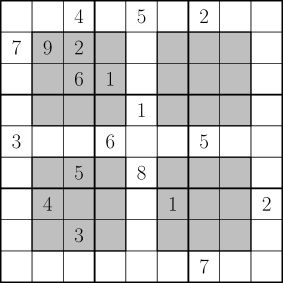
\includegraphics[width=0.45\textwidth]{NRC}
	b.
	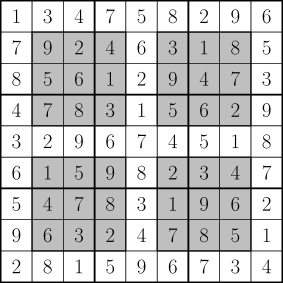
\includegraphics[width=0.45\textwidth]{NRC_solved}
	\end{center}
	\caption{\label{NRCout}The resulting graphic after processing the gss puzzle output with asymptote. a: The processed puzzle output. b: the processes solution output}
\end{figure}

\section{\label{util}Creating sudokus with gss}
To create new sudokus with gss you have to supply gss with a template sudoku, i.e. an input file describing a sudoku. The template sudoku is first solved by gss and subsequently randomized. After randomization gss eliminates elements again to create the new sudoku. For this procedure one needs a valid sudoku as a template. In some cases you may not have a valid sudoku (e.g. if you create a new sudoku layout you may not know a valid solution for the grid). In this case you can have gss try to fill your sudoku for you. There are two algorithms for filling sudokus. The first algorithm (invoked using the \texttt{-f} option) starts with an empty grid and using backtracking until a valid solution is found. This works well for standard size sudokus but for larger grids this method becomes unusable as it becomes too slow. In this case you can try fill the sudoku with an optimization algorithm (invoked with \texttt{-F}). Note, that not all sudoku structures you may come up with have a valid solution. The backtracking algorithm will tell you if no valid solution is found. However, the optimizer has no way of telling as it is not systematic in its search for a solution. If the optimizer fails you may have to try the backtracker to verify a solution exists. In the following two sections I discuss JigSawMRF, a random field generator to aid the creation of jigsaw sudokus and the MakeBook.sh script which demonstrates the creation of various types of sudokus. You can use the script as a tool to create puzzle books or study it to learn how to make your own sudokus with gss.


\subsection{\label{jig}JigSawMRF: A random field generator for jigsaw sudokus}
A common variety of sudokus are jigsaw sudokus where some blocks are irregularly shaped. Usually a jigsaw sudoku consists of some regular blocks, such as rows and columns, and irregular blocks. To obtain a somewhat playable sudoku the cells in an irregular block are generally all connected, which makes it possible to make clear graphical representation of the irregular blocks. Naturally, gss has no problem solving a jigsaw sudoku as we can simply define the irregular blocks with the \textless block\textgreater  or \textless matrix\textgreater  tags. However, gss cannot create a new jigsaw structure. To generate new jigsaw sudoku structures the utility JigSawMRF is provided. The JigSawMRF utility generates a random field, which separates a field into a number of equal sized and connected blocks.

The elements in the random fields JigSawMRF generate all have an ID number and a coordinate in an N dimensional space. The ID number can be used in gss to specify which cells belong to which block. The coordinates were introduced to aid the graphical representation of the field. The number of dimensions is at least one but can otherwise be chosen freely (so yes, you can create hyper dimensional jigsaw sudokus). 

The JigSawMRF program starts with a specification of the field, i.e. which elements are in it, and for each element, which elements are its neighbors. The elements are than assigned random "phases", i.e. are assigned to a random block. Then JigSawMRF iteratively swaps element phases until all elements of a specific phase are directly connected or connected via neighbors of the same phase.

The JigSawMRF program is called from the command line as follows:
\begin{verbatim}
JigSawMRF [options+arguments]
\end{verbatim}
The following options with arguments are supported:
\begin{description}
\item [\texttt{--rect, -r}] \hfill \\ Specify a rectangular field with rows and columns. This option must be followed by two numbers (N rows and M columns). With this option ech element in the field is connected with the elements above, below, left, and right to it (i.e. no diagonal connections). The elements are indexed in column mayor sequence.  
\item [\texttt{--custom, -c}] \hfill \\ Specify a field manually. Use this option to have full control over the field (e.g. non-rectangular fields). This option is followed by an input file-name where the field topology is specified. Each line in the file must have the format:
\begin{verbatim}
(<x>,<y>,..) <EL ID's>
\end{verbatim}
where, \verb|(<x>,<y>,...)| specifies the coordinate of each element in n dimensional space. You can provide an arbitrary number of dimensions provided all elements coordinates are specified with the same number of dimensions. The element ID's specify the neighbors of the element where the element ID's are numbered in the order of specification the file, starting at 1. 
\item [\texttt{--phases, -p}] \hfill \\ Specify the number of phases (blocks) in the field
\item [\texttt{--outp, -p}] \hfill \\ Output phases and coordinates. The output file contains N columns for the N dimensional coordinate, plus a column with phase and a column with the block size. The last column is for debugging purposes and can indicate if one block consists of several disjoint areas.
\item [\texttt{--outpe, -e}] \hfill \\ For each phase print the member element ID's. This data may be used to create the block definition in gss using the \textless block\textgreater  tag. 
\item [\texttt{--outb, -b}] \hfill \\ Export border points. For every two neighboring cells which are not a member of the same block, export the coordinate exactly between the two element coordinates.  
\item [\texttt{--verbose, -v}] \hfill \\ Specify the verbose level, L. If  L=0, the output is minimal, otherwise  JigSawMRF will print out every L-th iteration the 
overall progress and the minimum number of connected elements in a set, e.g., if this number if 1 it means there is at least one element which is not connected to any other element of the same block).
\item [\texttt{--offset, -o}] \hfill \\ Specify an offset value for element ID's. This affects the element ID numbers in all output data. This is sometimes useful, for example when only a part of a puzzle, with a specific range of element ID's is randomized.
\end{description}

\subsection{\label{book}MakeBook.sh: A script for creating sudoku books}
The script MakeBook.sh can create pdf's with puzzles and solutions for various types of sudokus. The script relies on pdflatex, asymptote, and naturally also on gss and JigSawMRF. The script is located in a directory with several gss input files and other shell scripts which are requires for the proper functioning of the script. Usage:
\begin{verbatim}
MakeBook.sh options+arguments]
\end{verbatim}
The following options with arguments are supported:
\begin{description}
\item [\texttt{--help, -h}] \hfill \\ Display a short help message
\item [\texttt{--level, -l}] \hfill \\ Specify the difficulty level
\item [\texttt{--type, -t}] \hfill \\ Specify the sudoku type
\item [\texttt{--out, -o}] \hfill \\ Specify the output file-name (pdf will be appended to the provided string)
\item [\texttt{--number, -n}] \hfill \\ Specify how many sudokus should be generated
\item [\texttt{--parallel, -p}] \hfill \\ In case the sudokus are large and/or of a high level, generating the sudokus may take some time. Use this flag to use more than one CPU when generating sudokus. This option relies on the GNU parallel program. 
\end{description}

The MakeBook.sh script knows several sudoku types. Samples of the sudoku types can be found below. The sudoku types are:
\begin{description}
\item [\texttt{STD}] \hfill \\Standard 9x9 sudoku:
\begin{center}
	
\includegraphics[width=0.45\textwidth]{STD}		
\end{center}
\item [\texttt{NRC}] \hfill \\ NRC sudokus, like a standard sudoku plus 4 extra blocks (marked in grey)
\begin{center}
	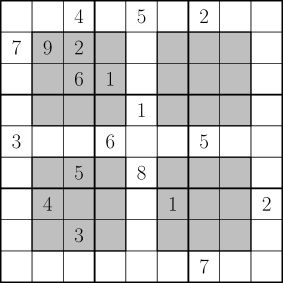
\includegraphics[width=0.45\textwidth]{NRC}		
\end{center}
\item [\texttt{NRCX}] \hfill \\ Like a NRC sudoku but with the two diagonals as additional blocks
\begin{center}
	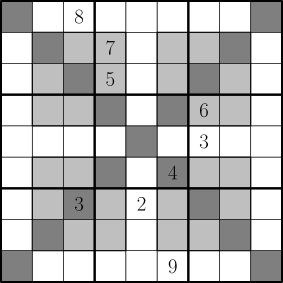
\includegraphics[width=0.45\textwidth]{NRCX}		
\end{center}
\item [\texttt{CUBE}] \hfill \\ Sudoku covering 3 faces of a cube. Each face consists of 4 4x4 blocks. Each row and each column extends over two faces.	
\begin{center}
	
\includegraphics[width=0.5\textwidth]{CUBE}	
\end{center}
\item [\texttt{JIGSAW}] \hfill \\ Jigsaw sudoku. Like a standard sudoku with irregular block shapes	
\begin{center}
	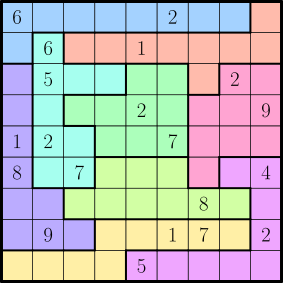
\includegraphics[width=0.45\textwidth]{jigsaw}	
\end{center}
\item [\texttt{JIGSAW-XL}] \hfill \\ Large jigsaw sudokus (16x16)	
\begin{center}
	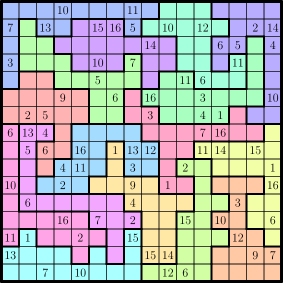
\includegraphics[width=0.45\textwidth]{jigsawxl}	
\end{center}
\item [\texttt{JIGCUBE}] \hfill \\ A jigsaw version of the CUBE type sudoku	
\begin{center}
	\includegraphics[width=0.5\textwidth]{bigjigcube}	
\end{center}
\item [\texttt{3DCUBE}] \hfill \\ Foldable 3D sudoku
\begin{center}
	
\includegraphics[width=0.5\textwidth]{3dcube}	
\end{center}
\item [\texttt{PARQ}]  \hfill \\ Parquet sudoku. Some elements cover more than one row and one column.	
\begin{center}
	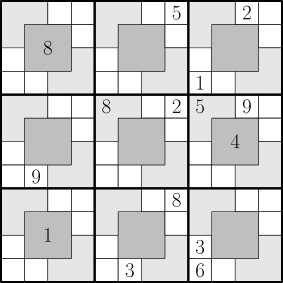
\includegraphics[width=0.45\textwidth]{parquet}	
\end{center}
\item [\texttt{LINKED}]  \hfill \\ A 9x9 sudoku with 9 extra color-coded blocks 	
\begin{center}
	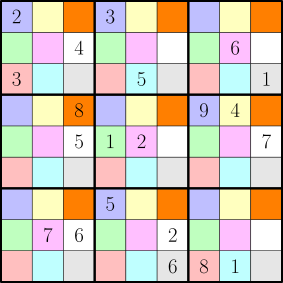
\includegraphics[width=0.45\textwidth]{linked}	
\end{center}
\end{description}


\appendix
\section{\label{NRC4ASY}Example input file for gss}
\begin{verbatim}
<size>81
<blocksize>9
<emptychar>0
<pattern>|.|
<standardblocks>
<matrix>
 +---------+-----------+---------+ 
 | .   . . | .   .   . | . .   . |
 |   +-----+---+   +---+-----+   |       
 | . | 1 1 | 1 | . | 2 | 2 2 | . |
 | . | 1 1 | 1 | . | 2 | 2 2 | . |
 +---+-----+---+---+---+-----+---+ 
 | . | 1 1 | 1 | . | 2 | 2 2 | . |
 |   +-----+---+   +---+-----+   |   
 | .   . . | .   .   . | . .   . |
 |   +-----+---+   +---+-----+   |       
 | . | 3 3 | 3 | . | 4 | 4 4 | . |
 +---+-----+---+---+---+-----+---+ 
 | . | 3 3 | 3 | . | 4 | 4 4 | . |
 | . | 3 3 | 3 | . | 4 | 4 4 | . |
 |   +-----+---+   +---+-----+   |  
 | .   . . | .   .   . | . .   . |
 +---------+-----------+---------+
<sudoku>
int[] f={|0|,|0|,|4|,|0|,|5|,|0|,|2|,|0|,|0|,
         |7|,|9|,|2|,|0|,|0|,|0|,|0|,|0|,|0|,
         |0|,|0|,|6|,|1|,|0|,|0|,|0|,|0|,|0|,
         |0|,|0|,|0|,|0|,|1|,|0|,|0|,|0|,|0|,
         |3|,|0|,|0|,|6|,|0|,|0|,|5|,|0|,|0|,
         |0|,|0|,|5|,|0|,|8|,|0|,|0|,|0|,|0|,
         |0|,|4|,|0|,|0|,|0|,|1|,|0|,|0|,|2|,
         |0|,|0|,|3|,|0|,|0|,|0|,|0|,|0|,|0|,
         |0|,|0|,|0|,|0|,|0|,|0|,|7|,|0|,|0|};
size(9cm);
int n = 3;
int N = n*n;
path cell = box((0,0),(1,1));
path supercell = box((0,0),(n,n));
for (int i=0;i<2;++i) {
    for (int j = 0; j < 2; ++j) {
        fill(shift((n+1)*i+1, (n+1)*j+1)*supercell, mediumgrey);
        draw(shift((n+1)*i+1, (n+1)*j+1)*supercell, black+linewidth(1pt));
    }
}
int k=0;
for (int i = 0; i < N; ++i) {
    for (int j = 0; j < N; ++j) {
        draw(shift(i, j)*cell, black+linewidth(0.5pt));
        if (f[k]>0)
            label(string(f[k]),p = fontsize(20pt), (i+0.5,j+0.5));
        k=k+1;
    }
}
for (int i = 0; i < n; ++i) {
    for (int j = 0; j < n; ++j) {
        draw(shift(n*i, n*j)*supercell, black+linewidth(2pt));
    }
}
\end{verbatim}

\end{document}
